% Shared preamble of the six stage reports (stages/README.md). Colours and notation are identical in every report.
\documentclass[11pt,a4paper]{article}
\usepackage[margin=2.2cm]{geometry}
\usepackage{amsmath,amssymb,booktabs,graphicx,xcolor,float,caption,subcaption,enumitem,longtable,array}
\usepackage[round]{natbib}
\usepackage[hidelinks]{hyperref}
\usepackage{fancyhdr}
\setlength{\emergencystretch}{2em}
\setlength{\parskip}{3pt}
\definecolor{roigreen}{RGB}{0,160,0}
\definecolor{artred}{RGB}{220,0,0}
\definecolor{maskblue}{RGB}{31,119,180}
\definecolor{ermgrey}{RGB}{110,110,110}
\definecolor{supported}{RGB}{0,120,0}
\definecolor{notsupported}{RGB}{190,0,0}
\newcommand{\ok}{\textcolor{supported}{\textbf{supported}}}
\newcommand{\no}{\textcolor{notsupported}{\textbf{not supported}}}
\newcommand{\mixed}{\textcolor{orange!80!black}{\textbf{partly supported}}}
\newcommand{\roi}{\textcolor{roigreen}{ROI}}
\newcommand{\na}{\textit{n/a}}
\newcommand{\registered}[1]{\textsf{registered before results (#1)}}
\newcommand{\posthoc}[1]{\textsf{post hoc (#1)}}
\pagestyle{fancy}\fancyhf{}\rhead{\small Where the Shortcut Sits --- stage reports}\lfoot{\small\leftmark}\rfoot{\small\thepage}
\newcommand{\stagebox}[1]{\noindent\colorbox{gray!12}{\parbox{\dimexpr\linewidth-2\fboxsep}{\small #1}}\par\medskip}

% generated by make_stage*.py from result files; do not edit
\providecommand{\sSixRemDermoscopymask}{$-0.049$ [$-0.083, -0.018$]}
\providecommand{\sSixRemDermoscopymte}{$-0.009$ [$-0.043, +0.024$]}
\providecommand{\sSixRemDermoscopymteprotect}{$-0.008$ [$-0.046, +0.028$]}
\providecommand{\sSixRemDermoscopybalanced}{$+0.213$ [$+0.183, +0.243$]}
\providecommand{\sSixRemDermoscopydfr}{$+0.196$ [$+0.157, +0.235$]}
\providecommand{\sSixRemDermoscopymtebalanced}{$+0.185$ [$+0.145, +0.224$]}
\providecommand{\sSixRemThyroidmask}{$+0.109$ [$+0.085, +0.133$]}
\providecommand{\sSixRemThyroidmte}{$+0.333$ [$+0.302, +0.364$]}
\providecommand{\sSixRemThyroidmteprotect}{$+0.393$ [$+0.347, +0.434$]}
\providecommand{\sSixRemThyroidbalanced}{$+0.388$ [$+0.360, +0.418$]}
\providecommand{\sSixRemThyroiddfr}{$+0.463$ [$+0.436, +0.492$]}
\providecommand{\sSixRemThyroidmtebalanced}{$+0.498$ [$+0.471, +0.524$]}
\providecommand{\sSixRemOvarianmask}{$+0.132$ [$+0.072, +0.196$]}
\providecommand{\sSixRemOvarianmte}{$+0.152$ [$+0.098, +0.203$]}
\providecommand{\sSixRemOvarianmteprotect}{$+0.175$ [$+0.116, +0.235$]}
\providecommand{\sSixRemOvarianbalanced}{$+0.290$ [$+0.248, +0.332$]}
\providecommand{\sSixRemOvariandfr}{$+0.310$ [$+0.263, +0.357$]}
\providecommand{\sSixRemOvarianmtebalanced}{$+0.321$ [$+0.271, +0.372$]}
\providecommand{\sSixRemCapsulemask}{$+0.084$ [$+0.055, +0.112$]}
\providecommand{\sSixRemCapsulemte}{$-0.042$ [$-0.076, -0.009$]}
\providecommand{\sSixRemCapsulemteprotect}{$+0.078$ [$+0.047, +0.107$]}
\providecommand{\sSixRemCapsulebalanced}{$+0.179$ [$+0.150, +0.205$]}
\providecommand{\sSixRemCapsuledfr}{$+0.234$ [$+0.199, +0.273$]}
\providecommand{\sSixRemCapsulemtebalanced}{$+0.258$ [$+0.221, +0.293$]}
\providecommand{\sSixNRemOK}{7}
\providecommand{\sSixNRem}{12}
\providecommand{\sSixNatRemPos}{5}
\providecommand{\sSixNatRemNeg}{8}
\providecommand{\sSixNatRemN}{20}
\providecommand{\sSixAuditN}{240}
\providecommand{\sSixAuditCohorts}{4}
\providecommand{\sSixAuditRated}{0}
\providecommand{\sSixAuditHash}{\texttt{4b5db1521f1fc214\ldots}}
\providecommand{\sSixExtAZeropos}{53}
\providecommand{\sSixExtAZeroneg}{1,954}
\providecommand{\sSixExttrapAAOnepos}{79}
\providecommand{\sSixExttrapAAOneneg}{2,057}
\providecommand{\sSixExttrapBAOnepos}{231}
\providecommand{\sSixExttrapBAOneneg}{18,685}
\providecommand{\sSixExtPatients}{2,056}
\providecommand{\sSixExtImages}{32,997}
\providecommand{\sSixSegBA}{0.929}
\providecommand{\sSixSegIoU}{0.601}
\providecommand{\sSixSegTau}{200}
\providecommand{\sSixExtX}{$+0.250$ [$+0.174, +0.327$]}
\providecommand{\sSixExttrapA}{$-0.064$ [$-0.128, -0.002$]}
\providecommand{\sSixExttrapB}{$+0.186$ [$+0.118, +0.249$]}
\providecommand{\sSixPagesMain}{22}
\providecommand{\sSixPagesSupplement}{18}
\providecommand{\sSixAbstractWords}{249}
\providecommand{\sSixTitle}{Masking cannot remove what is inside the region of interest: location-dependent shortcut mitigation across dermoscopy, ultrasound and capsule endoscopy}
\providecommand{\sSixAuditIntervals}{367}
\providecommand{\sSixAuditNumbers}{970}
\providecommand{\sSixAuditFailed}{0}
\providecommand{\sSixClaimN}{43}
\providecommand{\sSixClaimYes}{35}
\providecommand{\sSixClaimNo}{2}
\providecommand{\sSixClaimNA}{3}
\providecommand{\sSixClaimPartial}{3}
\providecommand{\sSixClaimPartialItems}{13, 18, 21, 33, 36}
\providecommand{\sSixRegFinal}{\texttt{c45d482}, 2026-09-28 00:35}
\providecommand{\sSixRegUmte}{\texttt{ee95f10}, 2026-09-26 20:14}
\providecommand{\sSixRegAbl}{\texttt{30f19c8}, 2026-09-27 14:15}
\providecommand{\sSixRegRevTwo}{\texttt{29cd0da}, 2026-09-27 18:56}
\providecommand{\sSixRegStat}{\texttt{4e9d44c}, 2026-09-27 09:37}

\title{\textbf{Stage 6 --- Remedies, label audit, external validation and the paper}\\[3pt]\large Where the Shortcut Sits: supervisor meeting 6 of 6}
\author{}
\date{Report generated from the repository on \today}
\begin{document}
\maketitle
\stagebox{\textbf{In one sentence.} What to do instead of masking depends on what carries the shortcut: annotation-free
erasure (U-MtE) repairs overlays that carry it in their pixels, label-based reweighting is needed when it is carried by
correlates, and no remedy improves on masking uniformly on unaltered data; the image audit that validates our artifact
labels is prepared for a clinician but not yet done; the dermoscopy result replicates on new patients; and the paper,
with every number traced to the regenerated results, is ready for the supervisor's review.}
% Shared notation. Each stage defines \notY, \notA, \notROI, \notCross, \notCI and \notExtra before \input-ing this
% file, so that a report only names the cohorts and quantities it has already introduced.
\section*{Notation}
\begin{tabular}{p{3.2cm}p{11.8cm}}
$Y\in\{0,1\}$ & diagnosis: \notY. \\
$A\in\{0,1\}$ & artifact present: \notA. \\
ROI & region of interest: \notROI; drawn in \textcolor{roigreen}{green}; artifacts in \textcolor{artred}{red}. \\
$r$ & overlap $|\text{artifact}\cap\text{ROI}|/|\text{artifact}|$. Trap~A: $r\ge0.5$ (artifact in the ROI); Trap~B: $r<0.1$ (outside). \\
Environments & training and correlated test $P(A{=}1\mid Y{=}1)=0.9$, $P(A{=}1\mid Y{=}0)=0.1$; reversed test 0.1/0.9; clean test: artifact independent of $Y$ (real artifacts: half of each class) or absent (synthetic artifacts). \\
ERM, mask & linear head on the frozen features of the original image / of the ROI-masked image. \\
Crossover & \notCross \\
CI & \notCI \\
$|\Delta p|$ & same-head counterfactual sensitivity: change of the predicted probability when the artifact is inserted into the same image. \\
\notExtra
\end{tabular}


\section{Where we are}
Stages~1--5 established the location law, its mechanism, its causal checks and its clinical consequences. This last
meeting covers what the thesis recommends in practice (the decision guide and the remedy tests of the primary family),
the evidence still missing (a clinician's audit of the automatic artifact labels), the external validation that was
feasible, the limitations, and the state of the paper: its structure, its number audit, the CLAIM checklist and draft
submission statements.

\section{Question}
\begin{enumerate}[label=\textbf{Q6\alph*},leftmargin=*]\itemsep1pt
\item Which remedy should replace or complement masking, and does any of them transfer to unaltered data?
\item How reliable are the automatic artifact labels that define ``inside'' and ``outside'' --- and how will a clinician
check them?
\item Does the main result hold on new patients from a different collection?
\item Is the paper ready to submit, and what must the author still decide?
\end{enumerate}
\paragraph{Design decisions} The remedies were demoted from a headline method to a \emph{decision guide} after the
second review: they are tested in the primary family, but the paper's claim is the location law, not a new method. The
image audit is \emph{blind} (neutral identifiers, cells hidden) and stratified by label so that precision and recall
can be estimated per location cell. External validation was run only if a pre-registered gate held (direct download,
licence, patient identifiers, masks, cell counts); datasets that need an agreement were listed, not used.

\section{Methods}
\paragraph{Remedies} ROI masking; U-MtE (mask-then-erase: after masking, erase from the frozen features the subspace
along which \emph{generic} synthetic overlays move the representation of masked images; no artifact annotation);
U-MtE protected (label directions protected from erasure); group balancing and DFR (need image-level artifact labels);
U-MtE with balancing. Primary tests: P2 (protected U-MtE $>$ mask), P3 (erasure $>$ augmentation with the same
overlays), P4 (U-MtE with balancing $>$ balancing), Trap~A, Holm over the 16-test family.
\paragraph{Image audit (Part B)} \sSixAuditN{} images: \sSixAuditCohorts{} cohorts $\times$ 3 cells (artifact inside the
ROI, outside it, artifact-free, by our automatic labels) $\times$ 20 (10 positive, 10 negative diagnosis), fixed seed,
the 518-px images the models saw. Each image and its overlay (ROI outline, automatic artifact mask) have a neutral
identifier; the reviewer fills artifact presence, location, mask correctness and ROI correctness in
\texttt{audit/review\_sheet.csv}. The key is kept outside the repository and fixed by its SHA-256
(\sSixAuditHash); \texttt{audit/analyse\_audit.py} computes precision, recall, location agreement, ROI correctness and,
with a second reviewer, Cohen's $\kappa$, and writes Table~\ref{tab:audit} of this report.
\paragraph{External validation (A4)} ISIC 2020 \citep{rotemberg2021isic2020}: lesion masks from the existing U-Net
(trained on ISIC 2018 only); hair/ruler masks from a segmenter trained only on the ISIC 2019 masks and frozen before
any ISIC 2020 image was scored (hair-free balanced accuracy \sSixSegBA, pixel IoU \sSixSegIoU); the ISIC 2019 trap
protocol unchanged with patient-disjoint folds.

\section{Experiments}
\begin{table}[H]\centering\scriptsize
\caption{Experiments of this stage and their registration documents (\texttt{docs/PREREGISTRATION\_<name>.md} or \texttt{docs/<name>.md}). Commit times are set by the committing machine and are not independent proof of order.}\label{tab:exp}
\begin{tabular}{p{3.1cm}p{2.1cm}p{2.4cm}p{3.2cm}p{3.3cm}}\toprule
Experiment & Status & Registration & First commit (local time) & Support criterion \\\midrule
U-I2E / U-MtE, protection, balancing, U7--U14 & \ok{} registered (with amendments before each run) & UNIVERSAL\_\allowbreak{}I2E & \texttt{ee95f10}, 2026-09-26 20:14 & per claim, CI; no gaming (clean loss $\le0.02$, corr $\ge$ rev $-0.02$) \\
Remedy tests P2--P4 in the 16-test family & \mixed{} tests registered; family grouped post hoc & STATISTICAL\_\allowbreak{}PLAN & \texttt{4e9d44c}, 2026-09-27 09:37 & Holm $p<0.05$, estimate $>0$ \\
Erasure-rank ablation & \ok{} registered & UMTE\_\allowbreak{}ABLATION & \texttt{30f19c8}, 2026-09-27 14:15 & descriptive \\
Encoder size (S2) & \ok{} registered & SCALE & \texttt{13303b0}, 2026-09-27 14:13 & protected U-MtE $>$ mask, CI \\
LaMa inpainting & \ok{} registered & INPAINT\_\allowbreak{}LAMA & \texttt{715b790}, 2026-09-27 09:41 & reported with CI, no direction \\
Text-prompted erasure (V1--V3) & \ok{} registered & TEXT\_\allowbreak{}PROMPT & \texttt{7877e8c}, 2026-09-27 12:21 & V1: text erasure $>$ mask \\
SLAS (S0--S6) & \mixed{} registration and localisation result share a commit & SLAS & \texttt{2d1ba20}, 2026-09-26 23:33 & S1: mask-then-suppress $>$ token masking \\
Chest drains (D1--D5) & \ok{} registered & CXR\_\allowbreak{}DRAIN & \texttt{3d0cffc}, 2026-09-27 03:29 & U-MtE $>$ mask, CI \\
Fine-tuning F1--F3 & \ok{} registered & FINETUNE & \texttt{7c8b466}, 2026-09-27 07:06 & mte\_ft $>$ mask, CI \\
Fine-tune, then erase & \ok{} registered & FT\_\allowbreak{}ERASE & \texttt{8ac7a7d}, 2026-09-27 14:20 & mte\_post $>$ mask\_post \\
Erase while fine-tuning (G1--G4) & \ok{} registered (amendments before running) & FT\_\allowbreak{}UMTE & \texttt{b7d7077}, 2026-09-27 14:52 & umte(\_cons)\_ft $>$ mask for both architectures \\
Leakage: embedding groups (P2--P4) & \ok{} registered & EMBEDDING\_\allowbreak{}GROUPS & \texttt{b0eda23}, 2026-09-27 13:55 & same sign and CI verdict \\
Natural data (N1, N2, N4) & \ok{} registered & NATURAL & \texttt{74bd243}, 2026-09-27 09:39 & protected U-MtE $\ge$ mask \\
Clinician image audit (prepared) & \ok{} registered & FINAL (Part B) & \texttt{c45d482}, 2026-09-28 00:35 & precision, recall, location agreement, $\kappa$ \\
\bottomrule\end{tabular}
\end{table}


\section{Results}
\subsection{Remedies and the decision guide}
Table~\ref{tab:rem} and Figure~\ref{fig:rem} compare the remedies in the in-ROI trap. Where the artifact carries the
shortcut in its pixels (calipers), U-MtE, which needs no annotation, repairs most of what masking leaves (thyroid
\sSixRemThyroidmte{} versus ERM, masking \sSixRemThyroidmask); with image-level artifact labels, U-MtE with balancing is
best (\sSixRemThyroidmtebalanced). Where the shortcut is carried by correlates of the artifact (dermoscopic hair), no
pixel-level method helps (U-MtE \sSixRemDermoscopymte) and reweighting is required (balancing \sSixRemDermoscopybalanced,
DFR \sSixRemDermoscopydfr). Where the artifact resembles the disease (capsule debris versus erosion fibrin), unprotected
erasure removes disease evidence (\sSixRemCapsulemte), protection repairs this (\sSixRemCapsulemteprotect), and
label-based methods are best (\sSixRemCapsulemtebalanced). In the primary family, \sSixNRemOK{} of \sSixNRem{} remedy
tests are supported after Holm correction (Table~\ref{tab:primrem}).
\begin{table}[H]\centering\scriptsize
\caption{Remedies in the in-ROI trap: change in reversed-test AUROC versus ERM (DINOv2, 5 seeds $\times$ 5 folds, crossed CIs). U-MtE needs no artifact annotation; balancing and DFR need image-level artifact labels.}\label{tab:rem}
\resizebox{\linewidth}{!}{\begin{tabular}{lcccccc}\toprule
Cohort (Trap A, in-ROI) & ROI masking & U-MtE & U-MtE protected & group balancing & DFR & U-MtE + balancing \\\midrule
Dermoscopy hair & $-0.049$ [$-0.083, -0.018$] & $-0.009$ [$-0.043, +0.024$] & $-0.008$ [$-0.046, +0.028$] & $+0.213$ [$+0.183, +0.243$] & $+0.196$ [$+0.157, +0.235$] & $+0.185$ [$+0.145, +0.224$] \\
Thyroid calipers & $+0.109$ [$+0.085, +0.133$] & $+0.333$ [$+0.302, +0.364$] & $+0.393$ [$+0.347, +0.434$] & $+0.388$ [$+0.360, +0.418$] & $+0.463$ [$+0.436, +0.492$] & $+0.498$ [$+0.471, +0.524$] \\
Ovarian calipers & $+0.132$ [$+0.072, +0.196$] & $+0.152$ [$+0.098, +0.203$] & $+0.175$ [$+0.116, +0.235$] & $+0.290$ [$+0.248, +0.332$] & $+0.310$ [$+0.263, +0.357$] & $+0.321$ [$+0.271, +0.372$] \\
Capsule debris & $+0.084$ [$+0.055, +0.112$] & $-0.042$ [$-0.076, -0.009$] & $+0.078$ [$+0.047, +0.107$] & $+0.179$ [$+0.150, +0.205$] & $+0.234$ [$+0.199, +0.273$] & $+0.258$ [$+0.221, +0.293$] \\
\bottomrule\end{tabular}}
\end{table}

\begin{figure}[H]\centering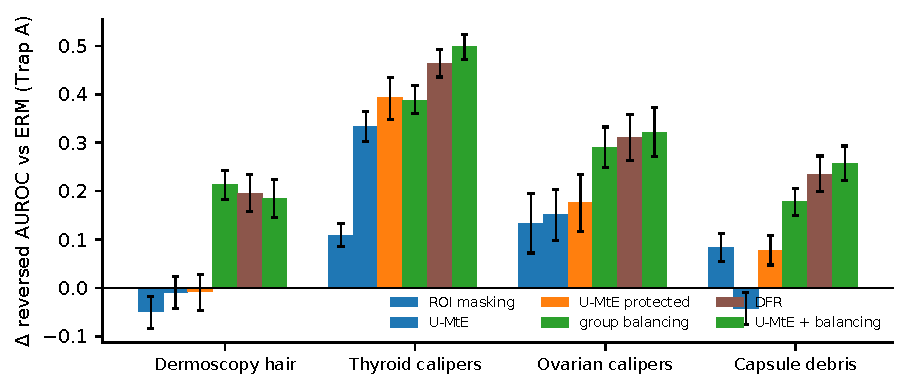
\includegraphics[width=0.9\linewidth]{figures/remedies.pdf}
\caption{Remedies in the in-ROI trap (change in reversed AUROC versus ERM, crossed 95\% CIs).}\label{fig:rem}\end{figure}
\begin{table}[H]\centering\scriptsize
\caption{Remedy tests of the 16-test primary family (Trap~A, reversed test).}\label{tab:primrem}
\begin{tabular}{lcccc}\toprule
Family & Cohort & Estimate [95\% CI] & $p$ (Holm, 16) & Supported \\\midrule
P2 U-MtE (protected) > mask & ISIC hair & $+0.042$ [$+0.024, +0.058$] & 0.0016 & \ok \\
P2 U-MtE (protected) > mask & Thyroid & $+0.283$ [$+0.237, +0.329$] & 0.0016 & \ok \\
P2 U-MtE (protected) > mask & Capsule & $-0.006$ [$-0.018, +0.006$] & 0.3486 & \no \\
P2 U-MtE (protected) > mask & Ovary & $+0.043$ [$+0.023, +0.065$] & 0.0016 & \ok \\
P3 erase > augment & ISIC hair & $+0.035$ [$+0.017, +0.055$] & 0.0016 & \ok \\
P3 erase > augment & Thyroid & $+0.215$ [$+0.189, +0.244$] & 0.0016 & \ok \\
P3 erase > augment & Capsule & $-0.139$ [$-0.158, -0.120$] & 0.0016 & \no{} (opposite) \\
P3 erase > augment & Ovary & $+0.035$ [$+0.003, +0.067$] & 0.1304 & \no \\
P4 U-MtE+balanced > balanced & ISIC hair & $-0.028$ [$-0.064, +0.007$] & 0.3486 & \no \\
P4 U-MtE+balanced > balanced & Thyroid & $+0.110$ [$+0.079, +0.142$] & 0.0016 & \ok \\
P4 U-MtE+balanced > balanced & Capsule & $+0.079$ [$+0.042, +0.115$] & 0.0016 & \ok \\
P4 U-MtE+balanced > balanced & Ovary & $+0.031$ [$-0.014, +0.077$] & 0.3486 & \no \\
\bottomrule\end{tabular}
\end{table}

\paragraph{On unaltered data no remedy transfers uniformly} On the natural test sets (Table~\ref{tab:natrem}), of
\sSixNatRemN{} remedy--test-set comparisons with masking, \sSixNatRemPos{} favour the remedy and \sSixNatRemNeg{}
favour masking; the rest are not significant. The decision guide therefore tells the reader which remedy fits which
regime and how to diagnose the regime (oracle artifact removal on a few annotated images; the theory's fitted
artifact--disease overlap), not which method to use everywhere.
\begin{table}[H]\centering\scriptsize
\caption{Remedies on the natural test sets (AUROC, all pairs, crossed CIs): no remedy improves on masking uniformly.}\label{tab:natrem}
\resizebox{\linewidth}{!}{\begin{tabular}{lcccc}\toprule
Natural test set & U-MtE $-$ mask & U-MtE protected $-$ mask & balancing $-$ mask & U-MtE + balancing $-$ mask \\\midrule
Thyroid (official split) & $+0.004$ [$-0.012, +0.020$] & $-0.021$ [$-0.034, -0.008$] & $-0.017$ [$-0.064, +0.030$] & $-0.005$ [$-0.023, +0.013$] \\
ISIC, BCN held out & $+0.007$ [$+0.004, +0.010$] & $-0.019$ [$-0.024, -0.014$] & $+0.022$ [$+0.012, +0.031$] & $+0.010$ [$+0.006, +0.015$] \\
ISIC, HAM held out & $+0.013$ [$+0.009, +0.017$] & $-0.006$ [$-0.016, +0.004$] & $-0.032$ [$-0.049, -0.013$] & $+0.018$ [$+0.009, +0.028$] \\
ISIC, MSK held out & $-0.008$ [$-0.014, -0.002$] & $-0.003$ [$-0.012, +0.006$] & $-0.018$ [$-0.041, +0.004$] & $-0.016$ [$-0.024, -0.008$] \\
Capsule (held-out frames) & $-0.005$ [$-0.011, +0.001$] & $-0.023$ [$-0.029, -0.017$] & $-0.086$ [$-0.109, -0.065$] & $-0.008$ [$-0.013, -0.001$] \\
\bottomrule\end{tabular}}
\end{table}

\begin{table}[H]\centering\scriptsize
\caption{The decision guide (paper, Sec.~``What carries the shortcut decides the fix'').}\label{tab:guide}
\begin{tabular}{p{3.4cm}p{3.6cm}p{4.2cm}p{3.6cm}}\toprule
Regime & Example & Recommended & Diagnostic \\\midrule
Overlay carries the shortcut in its pixels & calipers, rulers, tubes & mask, then U-MtE (no labels) or U-MtE with balancing (labels) & oracle removal of the artifact recovers most of the gap \\
Artifact resembles the pathology & capsule debris vs.\ fibrin & mask plus DFR; protected erasure if no labels & large fitted artifact--disease overlap \\
Shortcut carried by correlates & dermoscopic hair, chest drains & DFR or group balancing (labels needed) & oracle removal recovers little \\
Encoder ignores the out-of-ROI artifact & chest tube with RAD-DINO & masking unnecessary & reversed $\approx$ clean AUROC at no overlap \\
\bottomrule\end{tabular}
\end{table}

\subsection{The image audit}
The package is in \texttt{audit/} (Figure~\ref{fig:ex6} shows the kind of image the reviewer sees; the audit images
themselves are not reproduced here, to keep the review blind). Licence decisions per dataset are in
Table~\ref{tab:lic}: images whose redistribution is not confirmed are kept outside the repository and regenerated from the
original data by the sampling script. Reviewed rows so far: \sSixAuditRated{} of \sSixAuditN.
% PLACEHOLDER: replaced by `python audit/analyse_audit.py <filled sheet> [second sheet]` after the review
\begin{table}[H]\centering\caption{Image audit of the automatic labels (to be filled).}\label{tab:audit}
\fbox{\parbox{0.9\linewidth}{\centering\textbf{Audit not yet performed.} The table of precision, recall, location agreement, Cohen's $\kappa$ and ROI-mask correctness per cohort is written here by \texttt{audit/analyse\_audit.py} once the review sheet has been filled.}}
\end{table}

\begin{table}[H]\centering\scriptsize
\caption{Licence decisions for publishing images (\texttt{audit/LICENCES.md}); unclear means not published.}\label{tab:lic}
\begin{tabular}{p{3.6cm}p{4.0cm}p{2.8cm}p{4.2cm}}\toprule
Dataset & Licence (source) & Committed? & Attribution \\\midrule
ISIC 2018 Task 1/\allowbreak{}2, ISIC 2019 images (incl. HAM10000, BCN\_20000, MSK) & CC BY-NC 4.0 (challenge.isic-archive.com/\allowbreak{}data) & Yes (raw images) & ISIC Challenge datasets 2018/\allowbreak{}2019; Tschandl et al. 2018 (HAM10000); Combalia et al. 2019 (BCN\_20000); Codella et al. (MSK) \\
HAM10000 lesion segmentations & CC BY-NC 4.0 (Harvard Dataverse doi:10.7910/\allowbreak{}DVN/\allowbreak{}DBW86T) & Yes (as ROI outlines) & Tschandl et al. 2020 \\
ISIC 2019 hair/\allowbreak{}ruler masks (Wegley et al., Scholars' Mine doi:10.71674/\allowbreak{}man1-qa33) & no licence stated on the repository page & No — every overlay that draws these masks stays local & — \\
TN3K images, nodule masks; TNCD labels & not stated for the data; the GitHub repositories (TRFE-Net, ACL) license their *code* under MIT only & No — all thyroid images local & — \\
MMOTU OTU\_2d & CC BY 4.0 (figshare doi:10.6084/\allowbreak{}m9.figshare.25058690) & Yes & Zhao et al. 2022, MMOTU \\
SEE-AI project dataset & CC BY 4.0 (Kaggle `capsuleyolo/\allowbreak{}kyucapsule`, the project's account) & Yes & Yokote et al. 2023/\allowbreak{}2024, SEE-AI project \\
Capsule expert contamination masks & CC BY 4.0 (figshare 27645021) & Yes & figshare 27645021 \\
NIH ChestX-ray14 & not used in the audit or example figures & — & — \\
\bottomrule\end{tabular}
\end{table}


\subsection{External validation on new patients}
The search is recorded in \texttt{stages/EXTERNAL\_VALIDATION\_SEARCH.md}. ISIC 2020 met every condition: direct
download, CC BY-NC licence, patient identifiers, masks producible by our frozen models, and the cell-count gate
(hair-free melanomas \sSixExtAZeropos, Trap~A melanomas \sSixExttrapAAOnepos, Trap~B melanomas \sSixExttrapBAOnepos; every
cell at least 50). On \sSixExtImages{} images of \sSixExtPatients{} patients the crossover is \sSixExtX: masking harms
with hair on the lesion (\sSixExttrapA) and helps with hair beside it (\sSixExttrapB) (Table~\ref{tab:ext}). Thyroid
cohorts with patient identifiers either lack nodule masks (ThyUS2Path) or require an agreement (TN-SCUI 2020; Stanford
AIMI) and were not used.
\begin{table}[H]\centering\small
\caption{External validation on new patients (ISIC 2020; patient-disjoint folds; DINOv2; crossed CIs).}\label{tab:ext}
\resizebox{\linewidth}{!}{\begin{tabular}{lccc}\toprule
ISIC 2020, mask $-$ ERM & reversed test & correlated test & clean test \\\midrule
Trap A (hair on the lesion) & $-0.064$ [$-0.128, -0.002$] & $+0.068$ [$+0.040, +0.099$] & $+0.027$ [$-0.011, +0.066$] \\
Trap B (hair beside it) & $+0.186$ [$+0.118, +0.249$] & $-0.130$ [$-0.160, -0.100$] & $+0.005$ [$-0.049, +0.056$] \\
\bottomrule\end{tabular}}
\end{table}

\begin{figure}[H]\centering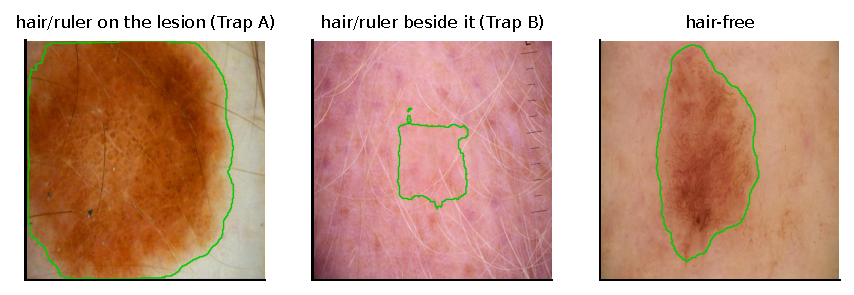
\includegraphics[width=0.85\linewidth]{figures/external_examples.pdf}
\caption{ISIC 2020 images from the external traps (CC BY-NC 4.0), with the lesion outline from the frozen U-Net
(\textcolor{roigreen}{green}); predicted hair/ruler masks are not drawn. Selection: a random image among the top quartile
of predicted hair/ruler area in each artifact cell (seed 20260928); any hair-free image.}\label{fig:ex6}\end{figure}

\subsection{The paper}
\paragraph{Title} \emph{\sSixTitle}. Target: \emph{Medical Image Analysis}. Main text \sSixPagesMain{} pages
(review format), supplement \sSixPagesSupplement{} pages; abstract \sSixAbstractWords{} words (limit 250).
\paragraph{Structure} Introduction; data and setup; the location law (controlled, real, transplant, matched, A2,
replication including ISIC 2020, chest-radiograph boundary); mechanism; theory (held-out prediction); consequences on
unaltered data (operating points, the post hoc thyroid subgroup labelled as exploratory confirmation); the decision
guide; robustness; discussion (including ``why this is not obvious'' and eight limitations).
\paragraph{Number audit} Every interval in the main text and supplement (the \verb|\input| tree of \texttt{main.tex}
and \texttt{supplement.tex}) must match an interval of a regenerated, crossed-bootstrap result file together with its
estimate; every other three-decimal number must occur in a result file. Result: \sSixAuditIntervals{} intervals and
\sSixAuditNumbers{} numbers checked, \sSixAuditFailed{} failed to trace.
\paragraph{CLAIM 2024} \sSixClaimN{} items: \sSixClaimYes{} yes, \sSixClaimPartial{} partial, \sSixClaimNo{} no,
\sSixClaimNA{} not applicable (partial or no: items \sSixClaimPartialItems; checklist in the supplement). The
remaining gaps are acquisition protocols the dataset providers did not release, the absence of external ultrasound and
capsule cohorts, and the clinician audit.

\subsection{Draft submission statements (for the author to confirm)}
\paragraph{Data availability} All datasets are public: ISIC 2018 and 2019 challenge data and ISIC 2020 (CC BY-NC 4.0),
HAM10000 lesion masks (CC BY-NC 4.0), the published ISIC 2019 hair/ruler masks, TN3K with TNCD labels, MMOTU (CC BY
4.0), SEE-AI and its expert contamination masks (CC BY 4.0), NIH ChestX-ray14 and RANZCR-CLiP (competition terms).
Derived masks, cohort files and all result files are in the repository; images are not redistributed where the
licence does not allow it.
\paragraph{Code availability} Code, pre-registrations with their commit history, result files and the scripts that
regenerate every table, figure and number are in the public GitHub repository (\texttt{hossam1999/\allowbreak Where\_\allowbreak shortcut\_\allowbreak sits}).
\paragraph{Ethics} Retrospective analysis of public, de-identified datasets released by their providers for research;
no new data were collected and no patient was contacted. The author should confirm with the institution whether a
formal waiver is required.
\paragraph{Use of AI assistance} The experiments, analysis code, reports and parts of the manuscript text were
produced with the assistance of an AI system (Claude, Anthropic) working under the author's direction; the author
designed the study, reviewed every result and is responsible for the content. The wording should follow the journal's
policy on generative-AI disclosure.

\section{What failed or changed}
\begin{itemize}[leftmargin=*]\itemsep1pt
\item \textbf{The clinician audit has not been done.} The package is ready; until it is, artifact-label validity rests
on the analysis agent's visual audit (Stage~3).
\item \textbf{No remedy transfers uniformly} to unaltered data; U-MtE was demoted from headline method to one option of
the decision guide. Three remedy tests of the primary family changed with the corrected bootstrap (Stage~4).
\item \textbf{External validation is dermoscopy only}; no thyroid cohort met the gate without an agreement or missing
masks.
\item \textbf{Chest-radiograph device and drain runs, LaMa inpainting and template erasure} could not be regenerated;
they appear as point estimates labelled ``not re-estimated''.
\item \textbf{Figures committed before the licence check} (\texttt{report/figures/data\_thyroid.png},
\texttt{report/figures/data\_isic.png}) conflict with the licence rule and need the author's decision.
\end{itemize}

\section{Conclusion}
\textbf{Supported.} A decision guide grounded in what carries the shortcut; external replication of the dermoscopy
crossover on new patients; a paper whose every interval traces to the corrected results. \textbf{Qualified.} The
remedies help in the trap environments but none transfers uniformly to unaltered data. \textbf{Not yet available.} A
clinician's audit of the artifact labels; external validation in ultrasound and capsule endoscopy.

\section{Questions for the supervisor}
\begin{enumerate}\itemsep1pt
\item Who should perform the image audit (two dermatologists and a sonographer?), and should it be completed before
submission?
\item Should the remedies stay in the paper as a decision guide, or move entirely to a second paper?
\item Is \emph{Medical Image Analysis} the right target, given the methodological emphasis, or would a clinical-AI venue
suit the operating-point results better?
\item Are the draft data-availability, ethics and AI-assistance statements acceptable to the institution?
\end{enumerate}

\section{Next stage}
Before submission: (i) run the clinician audit and replace Table~\ref{tab:audit} with the audit analysis script
(\texttt{audit/\allowbreak analyse\_\allowbreak audit.py}); (ii) decide on the figures that conflict with the licence rule; (iii) confirm the
submission statements; (iv) obtain the supervisor's decisions above; (v) push the final registration record and tag the
submitted version.

\bibliographystyle{plainnat}
\bibliography{../common/references}
\end{document}
